\section{Sistema perturbado y filtros}
Con el fin de tener un modelo que emule de una mejor manera el mundo real,
se decidío introducir diferentes perturbaciones al sistema, tanto en la
entrada, esto con el fin de reproducir el error introducido por los sensores
y eventualidades que pueden afectar el sistema, como en la salida, nuevamente
para simular los erroes de medida.

Las perturbaciones introducidas a la entrada, poseen una naturaleza aleatoria,
en particular se optó por utilizar un ruido blanco con periodo de
muestreo $0.1$ y potencia $0.01$, pues los sensores reales poseen errores
asociados a los cambios de voltaje, los cuales pueden ser modelas mediante un
ruido blanco.
La entrada perturbada se puede ver en la figura~\ref{fig:entrada-ruido}

\begin{figure}[t]
  \label{fig:entrada-ruido}
  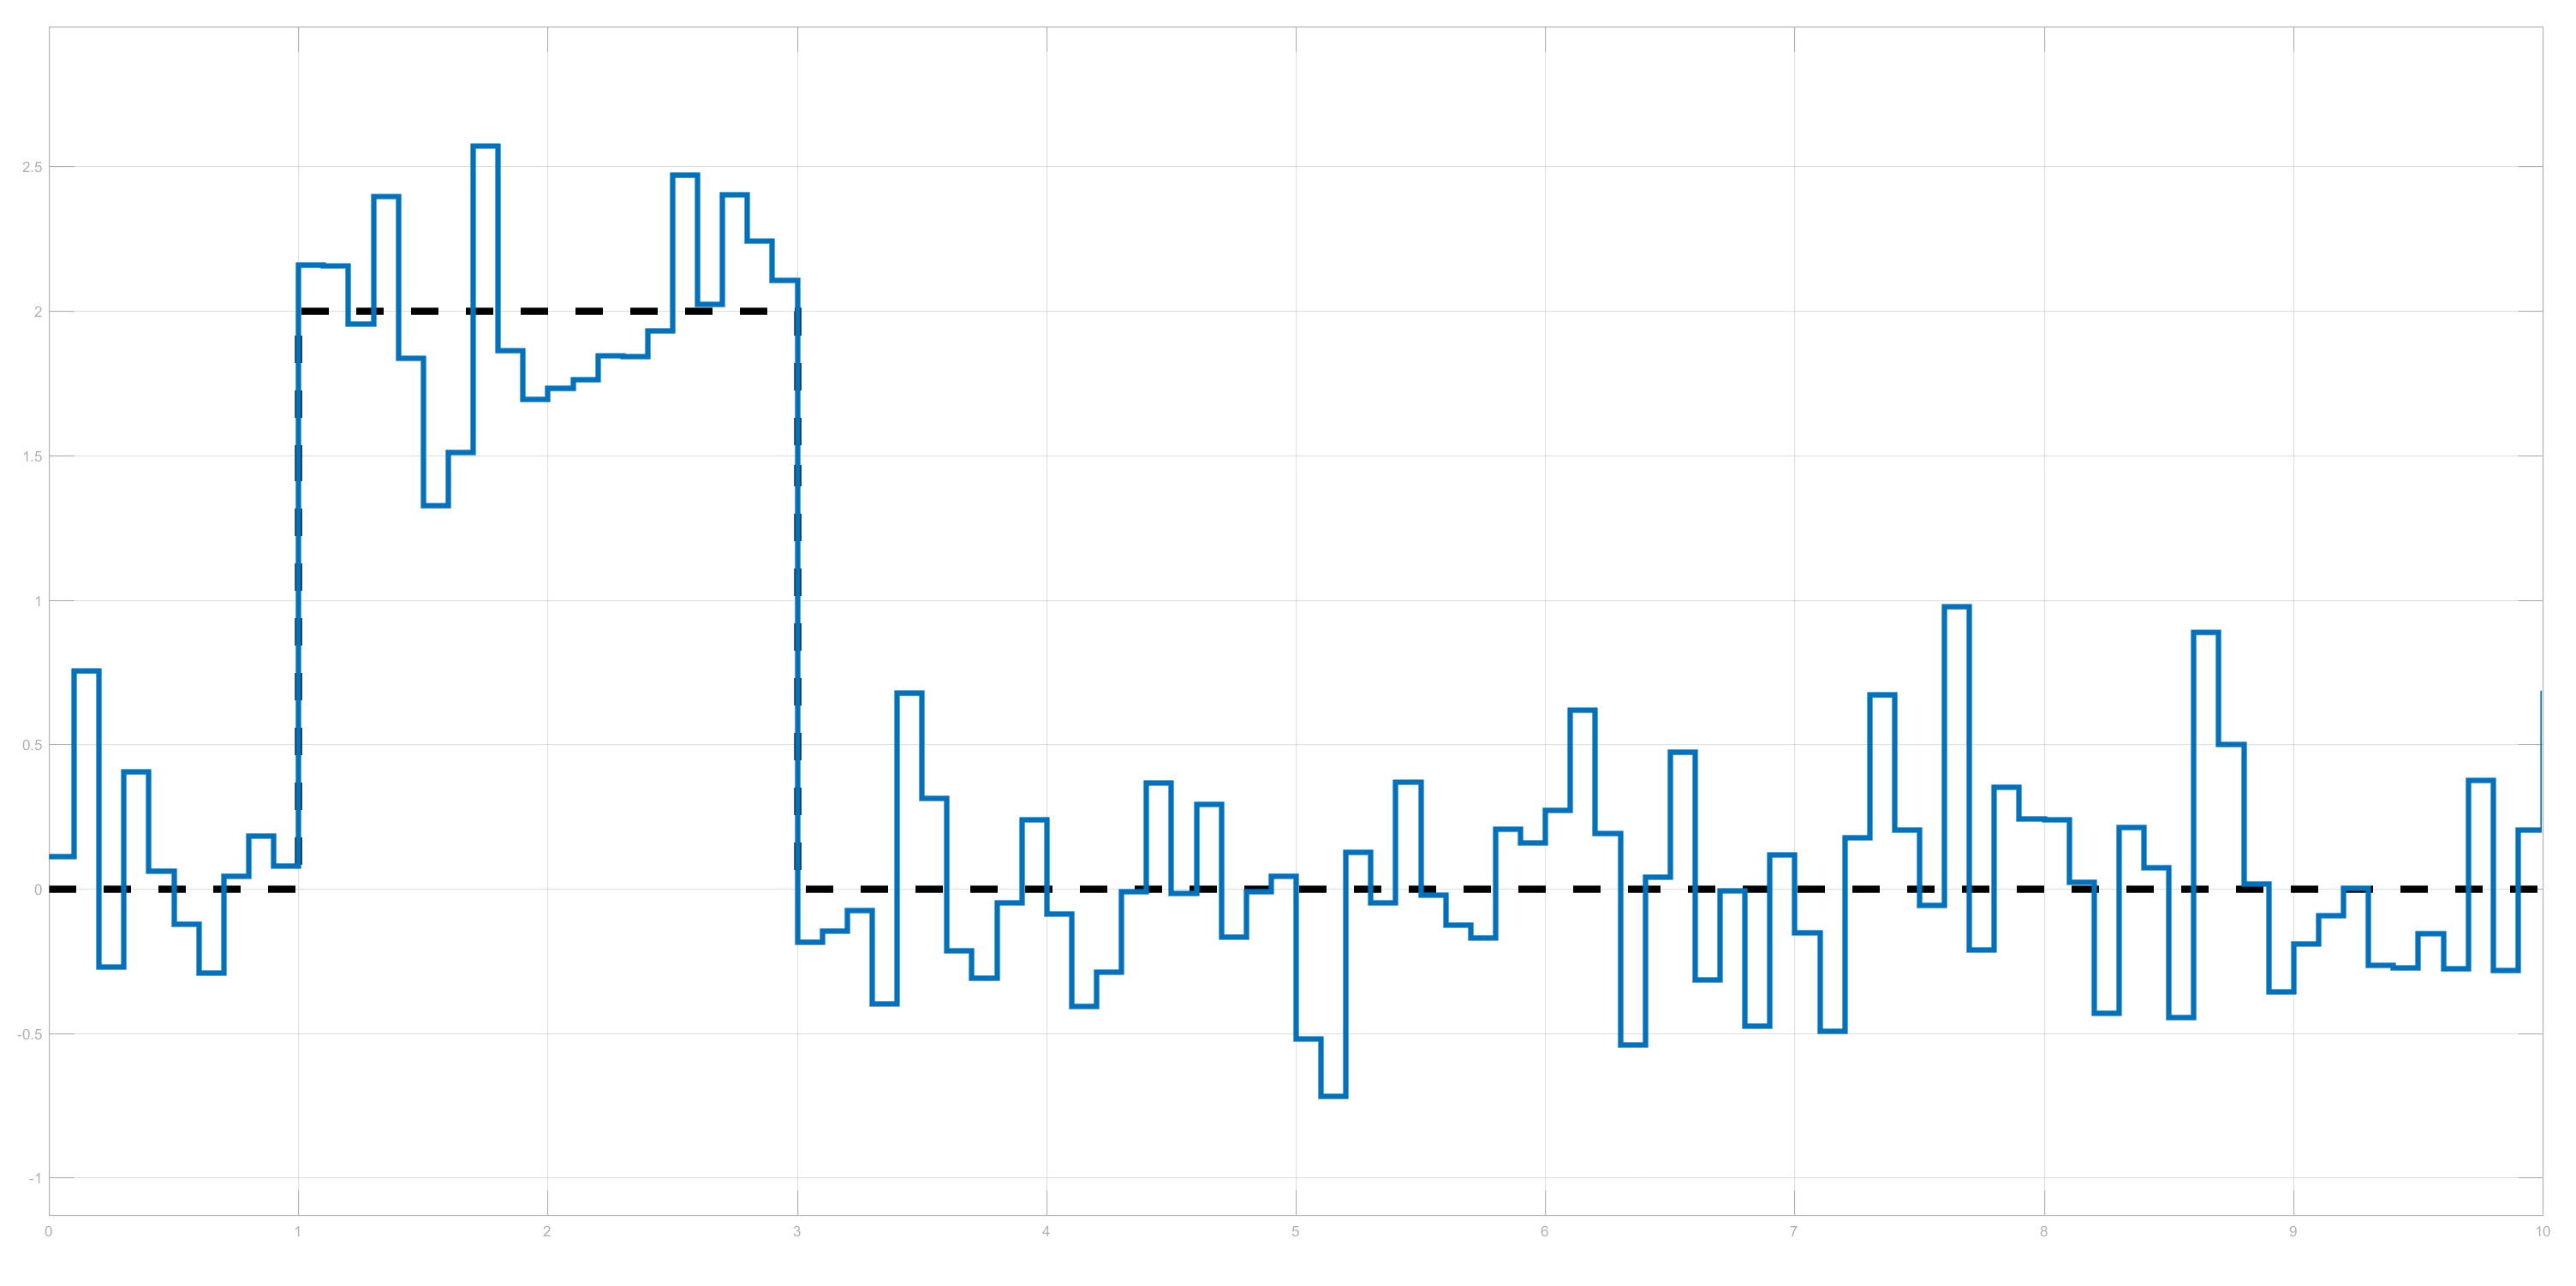
\includegraphics[scale=1]{Figuras/entrada}
  \caption{Señal de entrada perturbada.} 
\end{figure}

Adicionalmente, tambien fue introducido al sistema perturbaciones deterministas
de alta frecuencia esto con el fin de simular el posible deterioro de ciertas
componentes, pues si bien estos fenomenos son aleatorios, su impacto en el sistema
puede ser tratado localmente de manera determinista. En particular se optó por
considerar una señal computesta por la suma de señales senoidales de alta frecuencia.

Con el fin poseer un sistema mas robusto, se diseñó un filtro basabajas de primer orden,
el cual, como su nombre lo indica, se caracteriza por permitir el paso de las frecuencias
más bajas y atenuar las frecuencias mas altas.

La literatura señala que la funcion de transferencia de dicho tipo de filtros
son de la forma:
\[
\frac{1}{\tau s + 1}
\]
Donde $\tau $ es un parametro temporal que depende de la frecuencia que se desea
filtrar, en particular para nuestro problema se decidió escoger $\frac{1}{15}$.

Tanto en~\ref{fig:filtro-angle}, como en~\ref{fig:filtro-c} se pude observar la
respuesta temporal del sistema excitado con la entrada observada
en~\ref{fig:entrada-ruido}, perturbado y filtrado.

\begin{figure}[t]
  \label{fig:filtro-angle}
  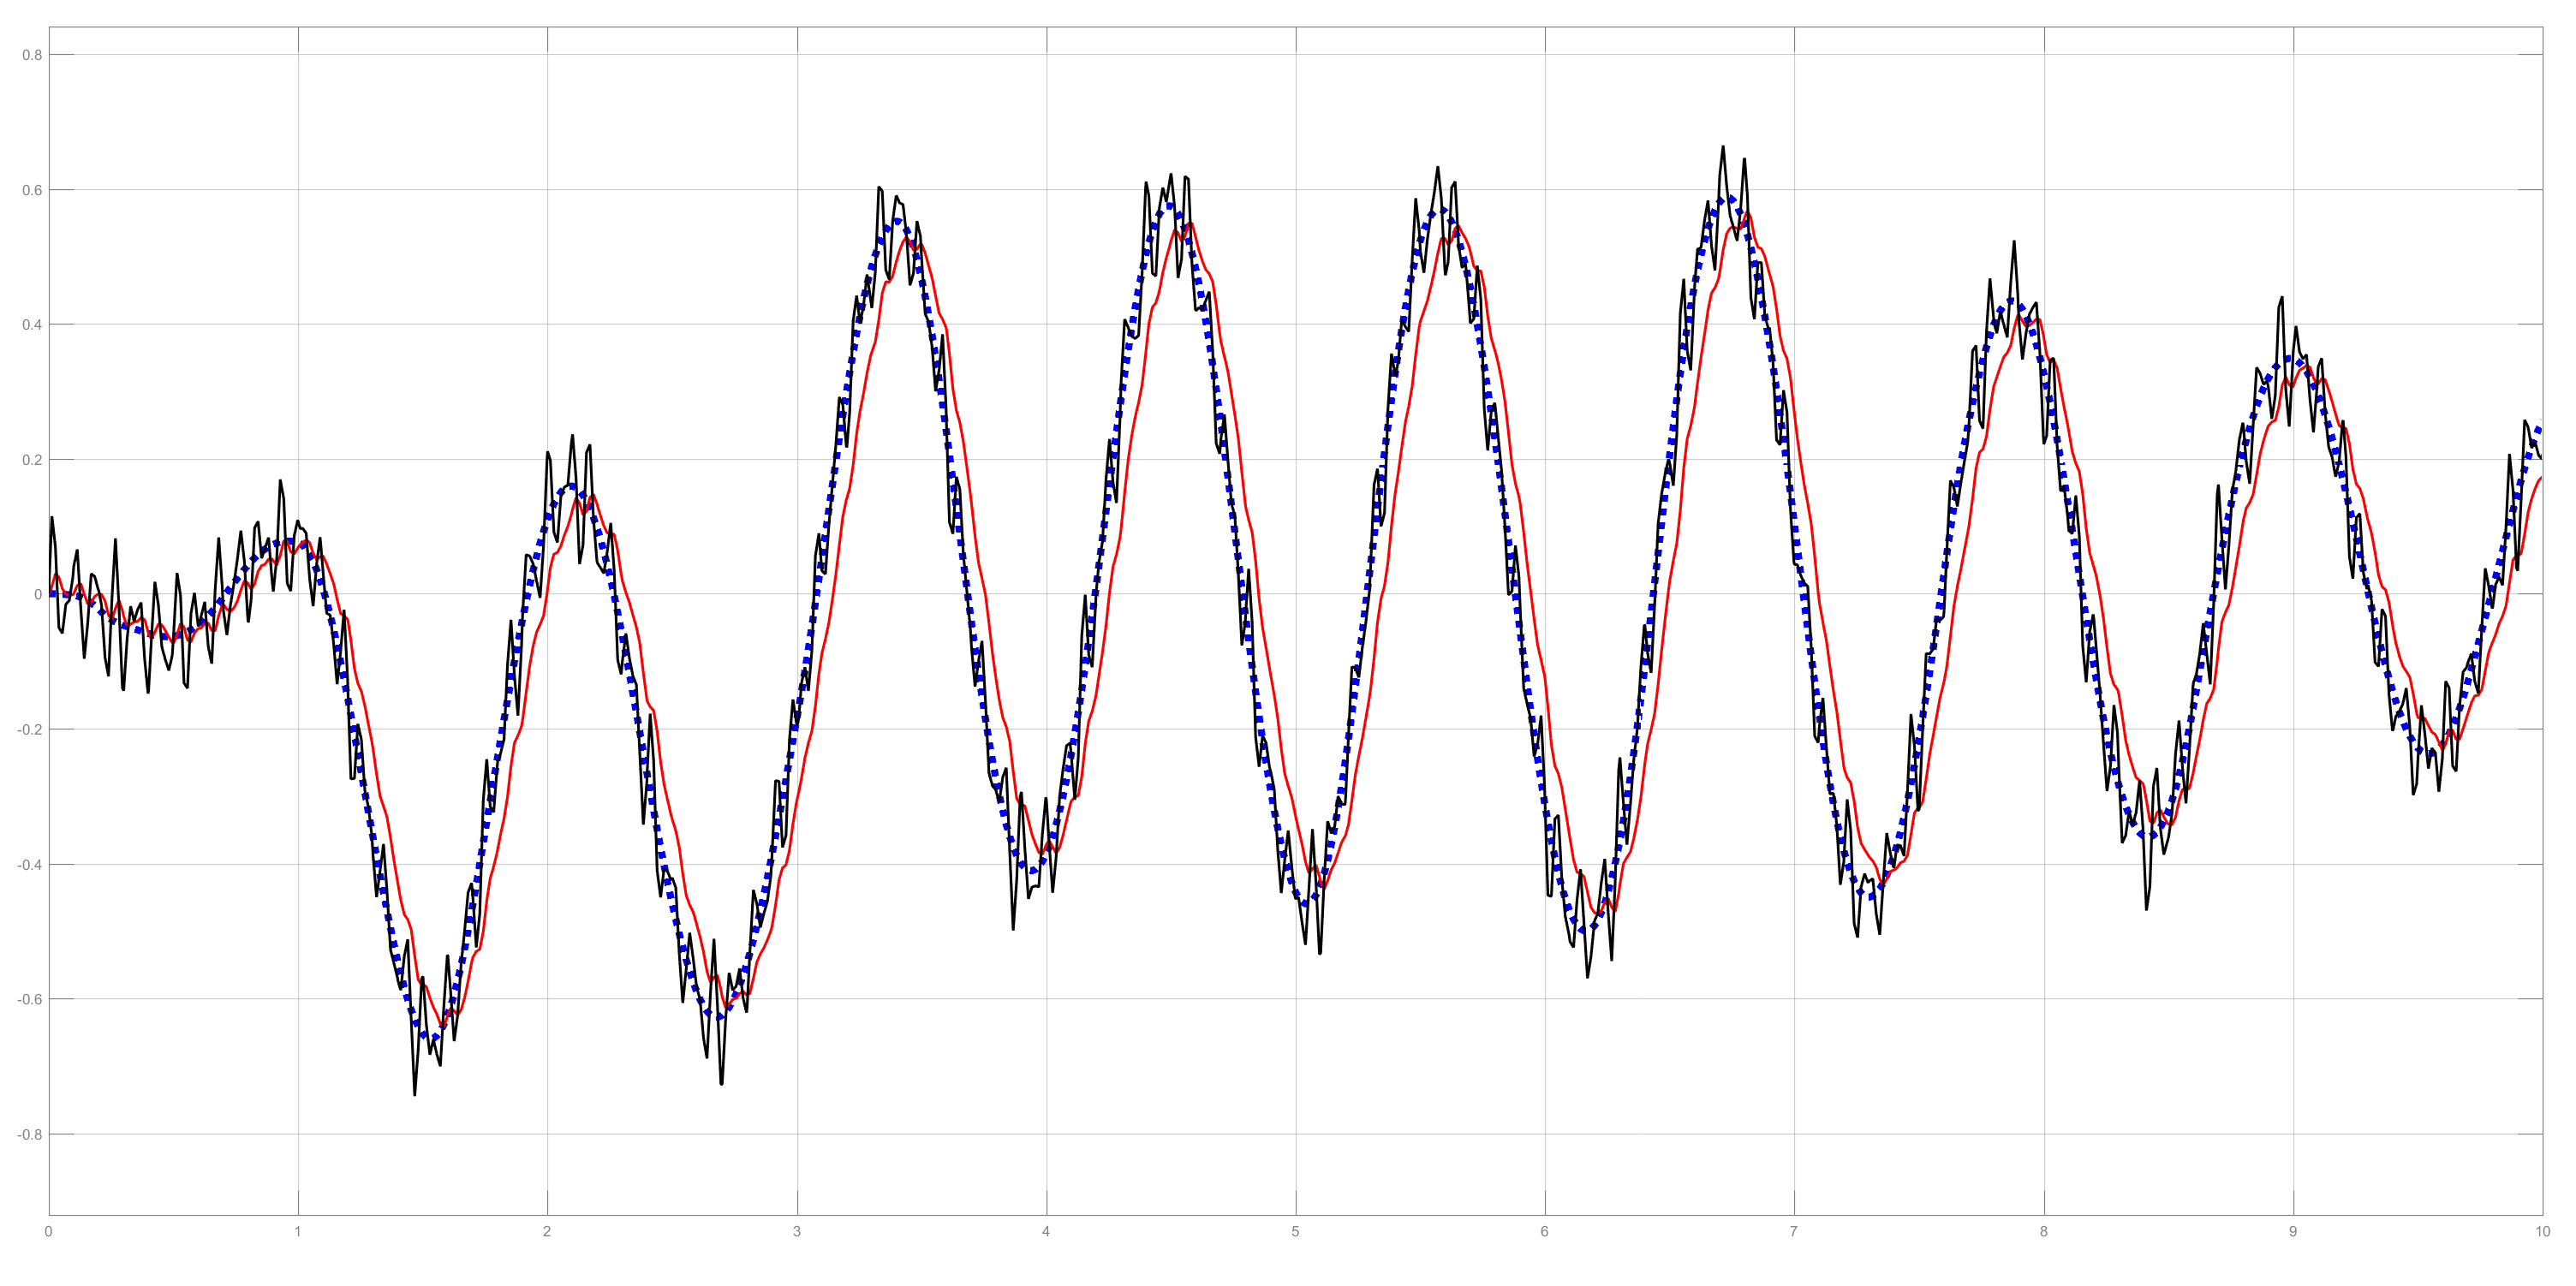
\includegraphics[scale=1]{Figuras/filtro-angle}
  \caption{Respuesta temporal del angulo perturbado y filtrado} 
\end{figure}

\begin{figure}[t]
  \label{fig:filtro-c}
  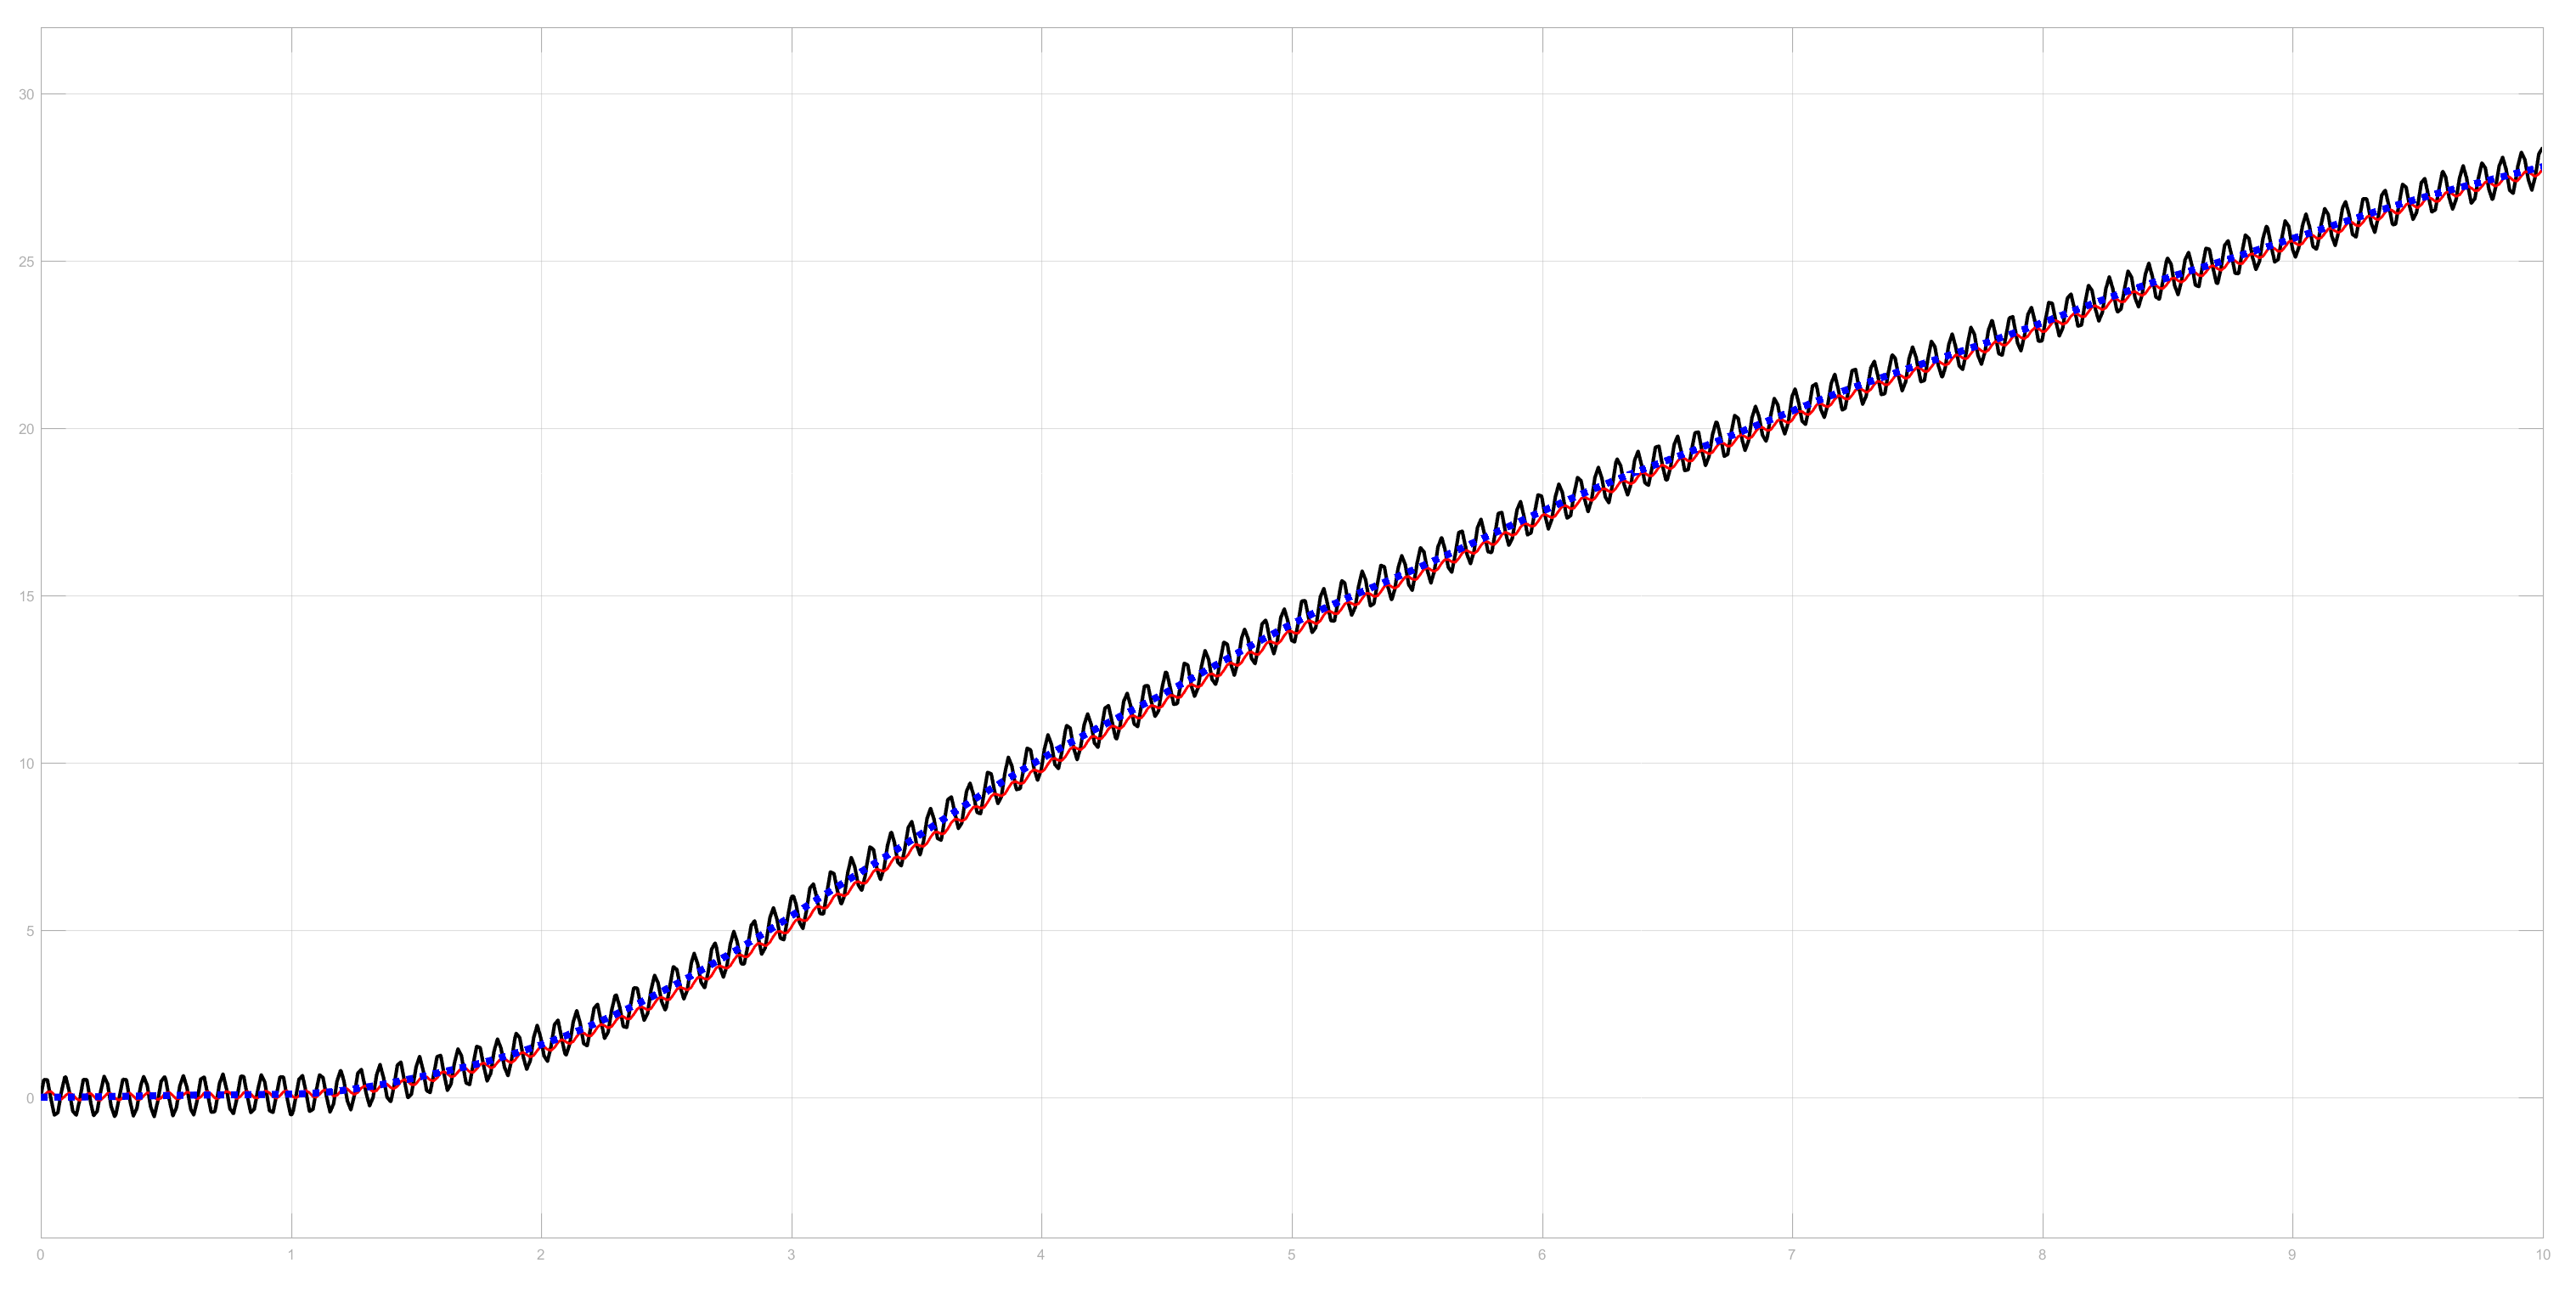
\includegraphics[scale=1]{Figuras/filtro-c}
  \caption{Respuesta temporal de la posicion perturbada y filtrada} 
\end{figure}